\chapter{Informed practical column sampling}

The previous chapter introduced the Nystr\"om approximation and showed why the choice of sampled columns matters. Uniform sampling is cheap but it does not use any information about which columns of the matrix are important. Exact leverage score sampling determines the importance of columns but it is too expensive as it requires the leading eigenvectors of the full kernel matrix which is the thing we are explicitly trying to avoid forming \citep{drineas2012fast,alaoui2015fast}. This chapter studies the middle ground: sampling methods that try to use importance information without paying the full cost of extracting spectral information.

The chapter has two sections. First, it introduces approximate leverage score sampling, where a small initial uniform sample is used to estimate column importance. Second, it introduces recursive ridge leverage score sampling, based on Algorithm 2 of \citet{musco2017recursive}. Chapter 5 compares these three sampling methods inside the KRR problem, in terms of approximation quality and prediction accuracy against runtime.


\section{Approximate leverage score sampling}

The heuristic used in this project is motivated by approximate leverage score estimation \citep{drineas2012fast,kumar2012sampling,gittens2016revisiting}. A simple version of approximate leverage score sampling is the following: First, sample a small number $l_0$ of columns uniformly. Second, use these columns to estimate which rows or columns of the kernel matrix are important. Finally, sample the remaining $l-l_0$ columns according to these estimated scores. For example, if $l=100$ and $l_0=5$, this means sampling $5$ columns uniformly and then sampling $95$ more columns according to approximate leverage scores.

Let
\[
I_0=\{i_1,\ldots,i_{l_0}\}
\]
be the initial uniformly sampled index set and define
\[
K_s=K_{:,I_0}\in\mathbb{R}^{n\times l_0}.
\]
We compute a thin singular value decomposition
\[
K_s=U_s\Sigma_s V_s^T.
\]
The columns of $U_s$ form an orthonormal basis for the column space found from the initially sampled columns. This small subspace is used as a rough approximation to the important part of the column space of the full matrix $K$. The approximate leverage score of row or column $i$ is computed as
\[
\hat s_i=\|U_s(i,:)\|_2^2
\] \citep{drineas2012fast,gittens2016revisiting}.
Similar to exact leverage scores, the approximate scores are then normalized to form a probability distribution
\[
p_i=\frac{\hat s_i}{\sum_{j=1}^n \hat s_j},
\]
and $l-l_0$ further columns are sampled according to these probabilities. The final index set is thus $I=I_0\cup I_1,$ where $I_1$ contains the extra sampled column indices. The Nystr\"om approximation is therefore
\[
\tilde K=K_{:,I}(K_{I,I})^\dagger K_{I,:}.
\]

We now discuss the diagnostics for approximate leverage score sampling to see whether the estimated scores are reliable by comparing them to the exact scores and also check how initial sampling affects the approximation.


\subsection{Comparison to exact leverage scores}
With this experiment, we aim to explain why approximate leverage sampling may or may not improve over uniform sampling. We randomly select $300$ observations from the standardized Superconductivity data and take the corresponding submatrix of the RBF kernel matrix
\[
K_{\mathrm{sub}}\in\mathbb{R}^{300\times300}.
\] The size $n=300$ is chosen to keep the exact eigendecomposition computationally cheap since we only use this experiment as a diagnostic comparison between exact and approximate leverage scores. Thus there are $300$ exact scores and each score measures importance relative to the leading $50$-dimensional eigenspace. For approximate leverage score sampling we use an initial uniform sample of $l_{\mathrm{ini}}=100$ columns. The approximate scores are then compared with the exact scores. For this comparison, only the first $r=50$ columns of $U_s$ are used when computing the approximate scores.

\begin{figure}[H]
\centering
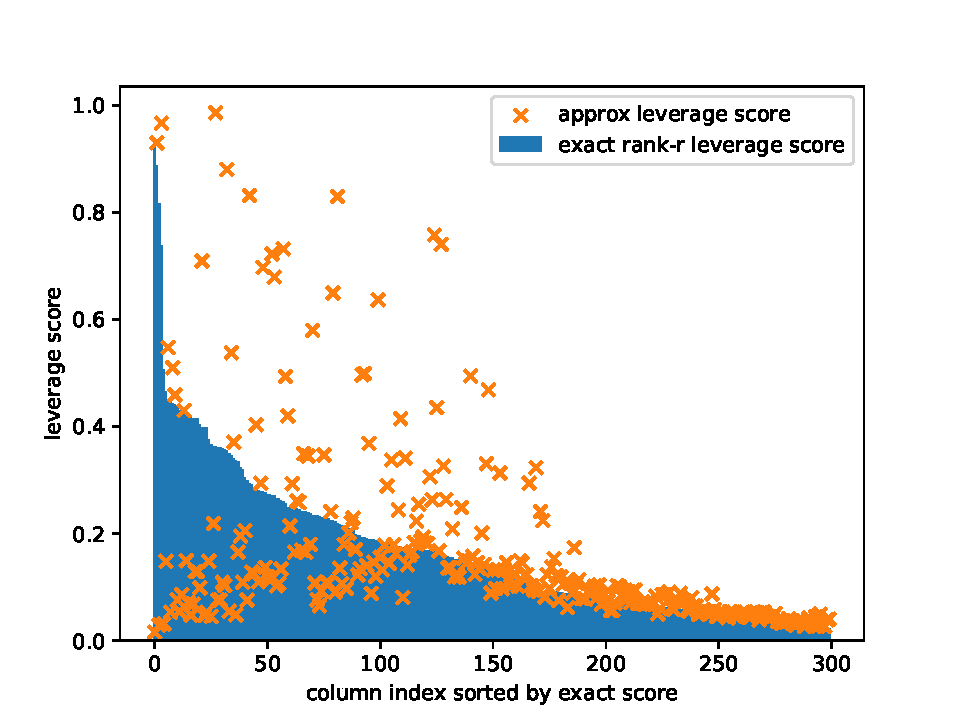
\includegraphics[width=0.78\textwidth]{Results/exact_vs_approx_leverage_scores.pdf}
\caption{Exact rank-$r$ leverage scores versus approximate leverage scores on a $300\times300$ kernel submatrix.}
\label{fig:evas}
\end{figure}
\FloatBarrier

Figure \ref{fig:evas} shows the exact scores as bars and the approximate scores as points, sorted by the exact score. If the approximation was perfect, the points would lie close to the tops of the bars. In this plot it seems that the approximate scores capture the broad scale but are very noisy. Some columns with high exact score are underestimated and some lower-score columns are overestimated. This shows why approximate leverage sampling is not guaranteed to beat uniform sampling in the final experiment as the score estimation step may contain a lot of error. 

\begin{figure}[H]
\centering
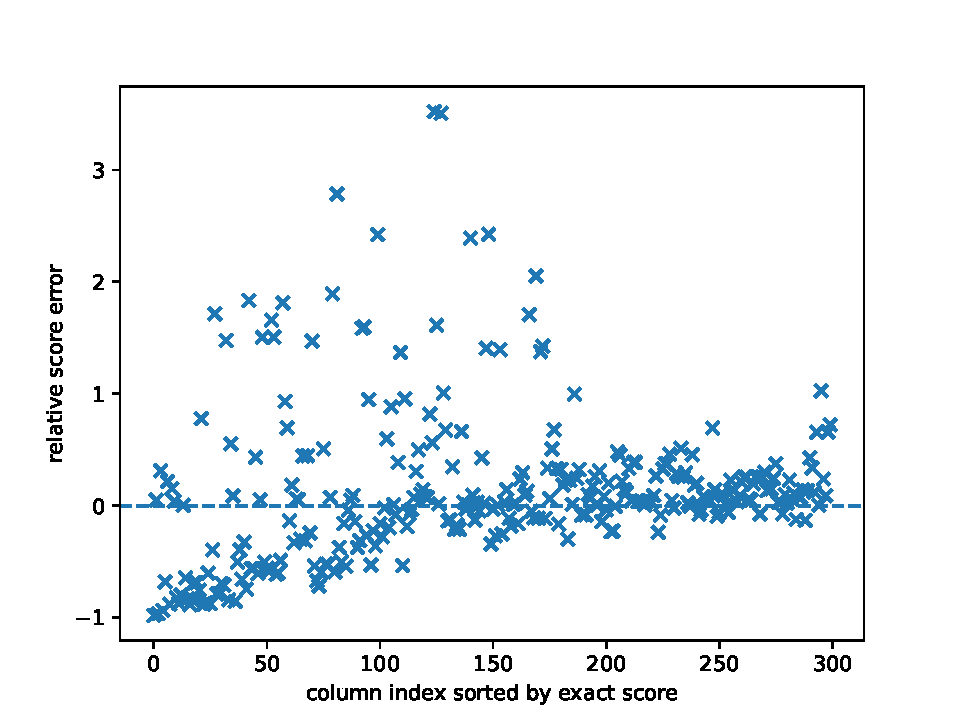
\includegraphics[width=0.78\textwidth]{Results/relative_leverage_score_error.pdf}
\caption{Relative error of approximate leverage scores compared with exact rank-$r$ scores.}
\label{fig:rse}
\end{figure}
\FloatBarrier

Figure \ref{fig:rse} shows the relative score error and clearly the errors are not uniformly small. This confirms our interpretation earlier, it seems that the initial sketch does not recover the leading eigenspace perfectly. Since the sampling probabilities are based on these scores, inaccurate scores can reduce the advantage over uniform sampling.

Next we vary $l_{\mathrm{ini}}$, with the target rank $r$ is fixed. Increasing $l_{\mathrm{ini}}$ gives more information about the column space, but it also makes the SVD step more expensive.

\begin{figure}[H]
\centering
\begin{minipage}{0.49\textwidth}
\centering
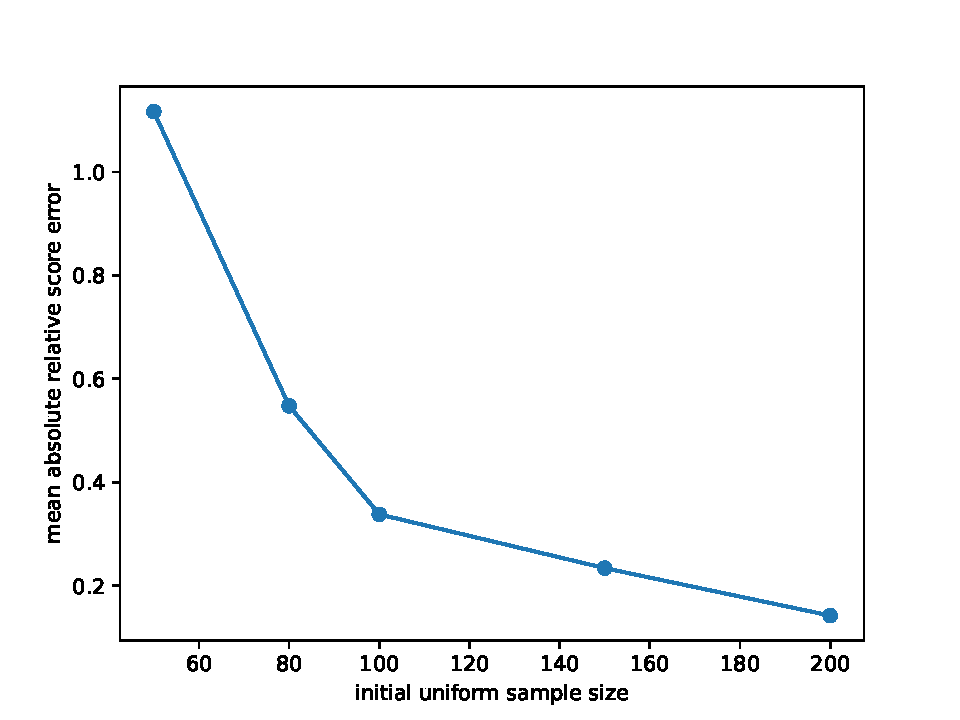
\includegraphics[width=0.98\textwidth]{Results/score_error_vs_initial_l.pdf}
\caption{Mean relative score error against the initial sample size.}
\label{fig:seil}
\end{minipage}
\hspace{0.005\textwidth}
\begin{minipage}{0.49\textwidth}
\centering
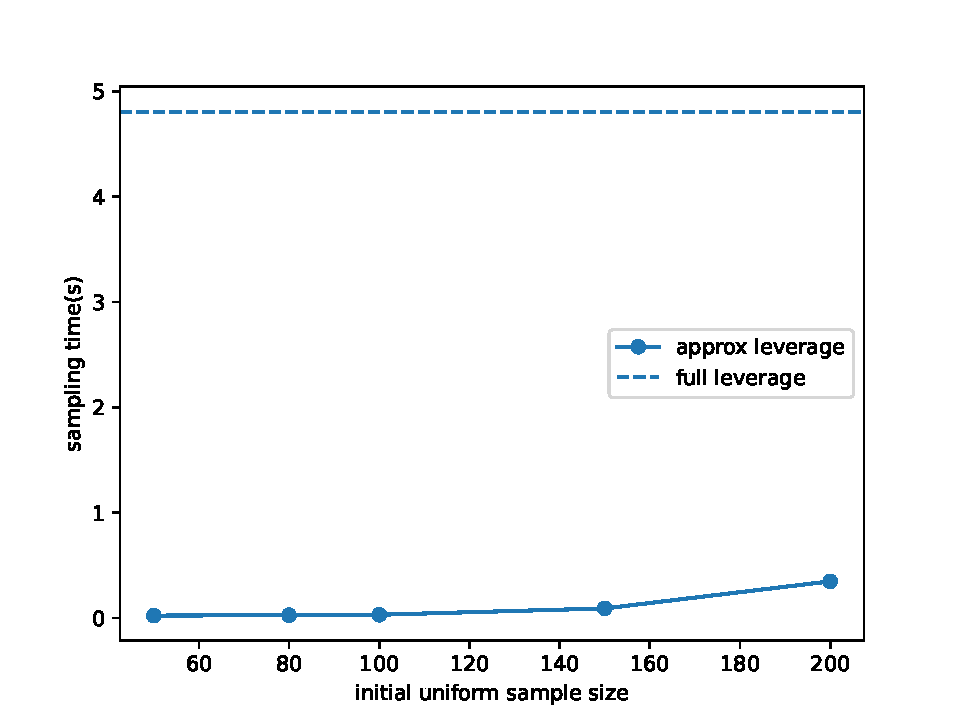
\includegraphics[width=0.98\textwidth]{Results/sampling_time_vs_initial_l.pdf}
\caption{Score estimation time against the initial sample size.}
\label{fig:stil}
\end{minipage}
\end{figure}
\FloatBarrier

Figures \ref{fig:seil} and \ref{fig:stil} show the expected trade off. As $l_{\mathrm{ini}}$ increases, the mean score error decreases. At the same time, the time required to estimate the scores increases. Next we investigate the effect of $l_{\mathrm{ini}}$ on the actual Nystr\"om approximation while the final number of sampled columns is fixed.

\subsection{Initial sample sizes and error}
Finally, the effect of $l_{\mathrm{ini}}$ is tested on the actual Nystr\"om approximation while the final number of sampled columns is fixed. We used a small subsample of size $n=2000$ and fixed the final number of sampled columns at $l=300$. The initial uniform sample size $l_{\mathrm{ini}}$ is varied from $50$ to $200$. The Nystr\"om approximation error is measured as the relative Frobenius norm error. The experiment was repeated five times with independent random column selections, and the mean error was reported.

\begin{figure}[H]
\centering
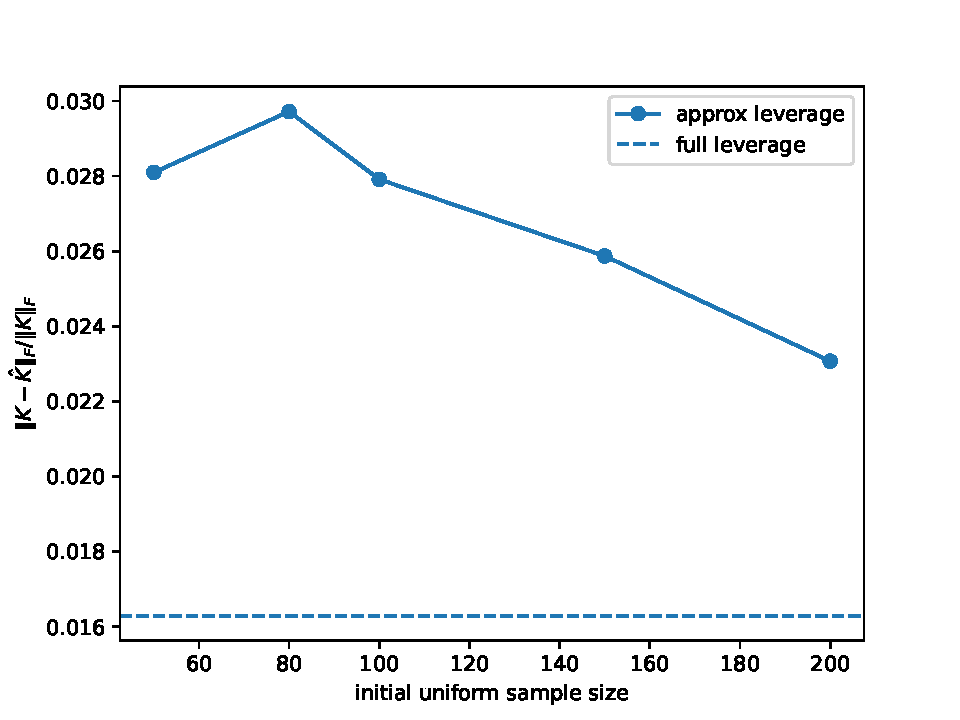
\includegraphics[width=0.72\textwidth]{Results/nystrom_error_vs_initial_l.pdf}
\caption{Mean Nystr\"om approximation error against the initial uniform sample size over five repetitions, with fixed final sample size.}
\label{fig:neil}
\end{figure}
\FloatBarrier

Figure \ref{fig:neil} shows that improving score accuracy does not automatically give a monotone improvement in the mean Nystr\"om error. The final sample size is fixed, so increasing $l_{\mathrm{ini}}$ also reduces the number of extra columns selected from the approximate scores. The result is roughly a trade off as a larger initial stage seems to give better score estimates, but it leaves less budget for the second stage. Repeated five-cycle experiment showed that the mean error still oscillates as $l_{\mathrm{ini}}$ increases, so the improvement remains nonmonotonic even after averaging over five repetitions.

\subsection{Limitations of approximate leverage sampling}

The approximate leverage method we used here is a crude practical compromise between uniform sampling and exact leverage score sampling which means it is not without limitations.

Indeed, the quality of these approximate scores depends entirely on whether the initial uniform sample captures the important directions of the full matrix. The method has the following dependency:
\[
\text{good initial sketch}
\Longrightarrow
\text{useful approximate scores}
\Longrightarrow
\text{good final sampling}.
\]
On the other hand,
\[
\text{bad initial sketch}
\Longrightarrow
\text{misleading approximate scores}
\Longrightarrow
\text{possibly worse final sampling}.
\]

This seems to create a circular difficulty. The purpose of leverage scores is to identify important columns, but the approximate leverage scores are themselves estimated from columns that were initially chosen uniformly. If an important direction is concentrated in a small number of columns and none of these columns is included in the initial sample, then this direction may not appear in the estimated subspace. The resulting approximate scores may therefore give low probability to exactly the columns that the method was intended to identify. Therefore the approximate leverage method may not be effective at all \citep{kumar2012sampling,gittens2016revisiting}.

There are three main situations in which this method may operate. First, if the true leverage scores are already close to uniform, then uniform sampling is likely to work well. In this case, the approximate leverage method adds the cost of constructing the initial sketch and computing its singular value decomposition without gaining much over the uniform baseline.

Second, if the leverage scores are nonuniform and the initial uniform sample captures the dominant directions sufficiently well, then the approximate scores may successfully identify important indices. The additional columns may then be sampled more effectively than under a uniform distribution.

Third, if the leverage scores are strongly nonuniform but the initial sample misses important directions, then the approximate scores can be inaccurate. In this case, the second sampling stage may fail to improve over uniform sampling and may even produce a worse landmark set.

The theoretical advantage of leverage score sampling therefore does not automatically apply to every approximate leverage procedure. Exact leverage score sampling has guarantees because its probabilities are constructed from the true leading eigenspace. Theorem 3.3 also permits approximate leverage-score probabilities, provided that
\[
p_i\geq\frac{\beta}{k}\|U_k(i,:)\|_2^2
\]
for some known $\beta\in(0,1]$. Thus, similar guarantees can also hold for approximate scores, but only when their sampling probabilities satisfy this lower bound. However, the simple two-stage method used here does not establish such a value of $\beta$. It should therefore be viewed as a heuristic method motivated by leverage score sampling \citep[Lemma~5]{gittens2016revisiting}. 

The difficulty above therefore motivates a more systematic approach. Rather than relying on one small uniform sample to approximate the important subspace immediately, recursive ridge leverage score sampling approximates through a sequence of progressively larger samples. Information obtained from a smaller sample is used to produce score estimates for a larger sample, and the recursion is designed so that the resulting probabilities provide theoretically controlled approximations to ridge leverage scores \cite{musco2017recursive}. We will see this in the next section.

\section{Recursive ridge leverage score sampling}

The previous section showed the main problems of the approximate leverage method. In this section we introduce Recursive ridge leverage score (RLS) sampling, which addresses this problem differently. Instead of asking one small sample to approximate the important subspace immediately, it estimates scores through a sequence of progressively larger sampled problems.

The algorithm used here is based on Algorithm 2 of \citet{musco2017recursive}. It first uses ridge leverage scores to provide a regularized measure of the importance of each data point. Then a recursive procedure approximates these scores without forming and decomposing the full kernel matrix.

\subsection{Ridge leverage scores and effective dimension}

Let $K\in\mathbb{R}^{n\times n}$ be a positive semidefinite kernel matrix. For a ridge parameter $\lambda_{\mathrm{RLS}}>0$, the ridge leverage score of point $i$ is defined as
\[
\ell_i^{\lambda_{\mathrm{RLS}}}(K) = [ K(K+\lambda_{\mathrm{RLS}}I)^{-1} ]_{ii}
\] \citep{alaoui2015fast}.

Ordinary rank-$r$ leverage scores use a fixed number of leading eigenvectors. Ridge leverage scores instead use a cut-off determined by $\lambda_{\mathrm{RLS}}$. To see this we look at the eigendecomposition of $K$ again, let
\[
K=U\Sigma U^T,
\]
where
\[
\Sigma=\operatorname{diag}(\eta_1,\ldots,\eta_n).
\]
Then
\[
K(K+\lambda_{\mathrm{RLS}}I)^{-1} = U\Sigma (\Sigma+\lambda_{\mathrm{RLS}}I)^{-1} U^T,
\]
and therefore
\[
\ell_i^{\lambda_{\mathrm{RLS}}}(K) = \sum_{j=1}^n \frac{\eta_j}{\eta_j+\lambda_{\mathrm{RLS}}} U_{ij}^2.
\]
The factor $\frac{\eta_j}{\eta_j+\lambda_{\mathrm{RLS}}}$ determines how strongly the $j$-th spectral direction contributes to the score. If $\eta_j\gg\lambda_{\mathrm{RLS}}$, then this factor is close to $1$. If $\eta_j\ll\lambda_{\mathrm{RLS}}$, then it is close to $0$. Thus the method controls how much information is kept by controlling $\lambda_{\mathrm{RLS}}$ \citep{alaoui2015fast,musco2017recursive}.

The sum of the ridge leverage scores is called the $\emph{effective dimension}$:
\[
d_{\mathrm{eff}}^{\lambda_{\mathrm{RLS}}} = \sum_{i=1}^n \ell_i^{\lambda_{\mathrm{RLS}}}(K) = \operatorname{tr} ( K(K+\lambda_{\mathrm{RLS}}I)^{-1} ).
\]
Using the eigendecomposition, this becomes
\[
d_{\mathrm{eff}}^{\lambda_{\mathrm{RLS}}} = \sum_{j=1}^n \frac{\eta_j}{\eta_j+\lambda_{\mathrm{RLS}}}.
\]

The effective dimension is not necessarily an integer. It measures the approximate number of spectral directions that remain important at the chosen $\lambda_{\mathrm{RLS}}$. A smaller $\lambda_{\mathrm{RLS}}$ keeps more directions and gives a larger effective dimension. A larger $\lambda_{\mathrm{RLS}}$ gets rid of more directions and gives a smaller effective dimension \citep{zhang2005learning,alaoui2015fast,musco2017recursive}.

Suppose that overestimates of the ridge leverage scores
\[
\widetilde\ell_i^{\lambda_{\mathrm{RLS}}} \geq \ell_i^{\lambda_{\mathrm{RLS}}}(K)
\]
are available. Using overestimates is important because it prevents an important point from being left out due to having a lower sampling probability than its exact ridge leverage score would require. Given these estimates, point $i$ is sampled independently with probability
\[
p_i = \min\left\{1,\; 16\widetilde{\ell}_i^{\lambda_{\mathrm{RLS}}} \log\left(\frac{ \sum_{j=1}^n \widetilde{\ell}_j^{\lambda_{\mathrm{RLS}}} }{\delta }\right)\right\},
\]
where $\delta$ is a failure probability parameter.

Since every point is sampled independently, the number of selected columns is random rather than fixed in advance. Let
\[
Z_i =
\begin{cases}
1, & \text{if point } i \text{ is selected},\\
0, & \text{otherwise}.
\end{cases}
\]
Then the total number of selected columns is
\[
l = \sum_{i=1}^n Z_i.
\]
Since point $i$ is selected with probability $p_i$, we have
\[
\mathbb{E}[Z_i] = p_i.
\]
Thus
\[
\mathbb{E}[l] = \sum_{i=1}^n p_i.
\]
For exact ridge leverage scores, \citet{musco2017recursive} show that
\[
\sum_{i=1}^n p_i = \mathcal{O}\left(d_{\mathrm{eff}}^{\lambda_{\mathrm{RLS}}}\log\left(\frac{d_{\mathrm{eff}}^{\lambda_{\mathrm{RLS}}}}{\delta}\right)\right).
\]
Thus the expected number of selected columns is controlled by the effective dimension. The recursive algorithm later achieves a corresponding high-probability bound on $l$ while avoiding the direct computation of the exact scores.

The remaining difficulty is that the exact ridge leverage scores, and hence the overestimates, cannot be computed cheaply from the full expression much like the exact leverage scores. Algorithm 2 of \citet{musco2017recursive} avoids this cost by recursively estimating the scores.

\subsection{Recursive approximation of the scores}

We now describe Algorithm \ref{alg:1} as below from \citet{musco2017recursive} where it estimates the scores recursively.

\begin{algorithm}[ht!]
\caption{RecursiveRLS-Nystr\"om}
\label{alg:1}
\begin{algorithmic}[1]

\Require Data points $x_1,\ldots,x_m\in\mathcal{X}$, kernel function $K:\mathcal{X}\times\mathcal{X}\rightarrow\mathbb{R}$, ridge $\lambda>0$, failure probability $\delta\in(0,1/32)$

\Ensure Weighted sampling matrix $S\in\mathbb{R}^{m\times s}$

\If{$m\leq 192\log(1/\delta)$}
    \State \Return $S:= I_{m\times m}$
\EndIf

\State Let $\overline{\mathcal{S}}$ be a random subset of $\{1,\ldots,m\}$, where each $i$ is included independently with probability $1/2$

\Statex \Comment{Let $\overline{X}=\{x_{i_1},x_{i_2},\ldots,x_{i_{|\overline{\mathcal{S}}|}}\}$, where $i_j\in\overline{\mathcal{S}}$}

\Statex \Comment{Let $\overline{S}=[e_{i_1},e_{i_2},\ldots,e_{i_{|\overline{\mathcal{S}}|}}]$ be the corresponding sampling matrix}

\State $\widetilde{S}:=\Call{RecursiveRLS-Nystr\"om}{\overline{X},K,\lambda,\delta/3}$

\State $\widehat{S}:=\overline{S}\widetilde{S}$

\State $\displaystyle \widetilde{\ell}_i^{\lambda}:=\frac{3}{2\lambda}\left(K-K\widehat{S}\left(\widehat{S}^{T}K\widehat{S}+\lambda I\right)^{-1}\widehat{S}^{T}K\right)_{ii}$ for every $i\in\{1,\ldots,m\}$

\Statex \Comment{By Lemma 6 of \citet{musco2017recursive}, equals $\frac{3}{2\lambda}(B(B^T\widehat{S}\widehat{S}^TB+\lambda I)^{-1}B^T)_{ii}$. $K$ denotes the kernel matrix for the points $\{x_1,\ldots,x_m\}$ and kernel function $K$}

\State $\displaystyle p_i:=\min\left\{1,\;16\widetilde{\ell}_i^{\lambda}\log\left(\frac{\sum_{i=1}^{m}\widetilde{\ell}_i^{\lambda}}{\delta}\right)\right\}$ for each $i\in\{1,\ldots,m\}$

\State Initialize the weighted sampling matrix $S$ as empty

\For{$i=1,\ldots,m$}
    \State With probability $p_i$, append the column $\dfrac{1}{\sqrt{p_i}}e_i$ to $S$
\EndFor

\State \Return $S$

\end{algorithmic}
\end{algorithm}

Consider one call of the algorithm on a set of $m$ data points.

\begin{enumerate}
\item If the index set is small enough, the recursion stops and returns all current points.
\item Otherwise each current point is included independently with probability $1/2$. This produces a uniformly sampled index set containing approximately half of the current points.
\item The same recursive algorithm is applied to this smaller index set. The returned weighted sample gives a compact approximation of the half-sized index set.
\item This approximation is lifted back to the current index set and used to estimate the ridge leverage score of every current point.
\item The current points are sampled according to the resulting probabilities $p_i$.
\end{enumerate}

The base case in Algorithm \ref{alg:1} is $m\leq 192\log(1/\delta)$. In this case the method returns the identity matrix, which means that all current points are retained. At every recursive call, the failure-probability parameter is changed from $\delta$ to $\delta/3$.

Now suppose that the recursive call on the smaller index set has returned a weighted sampling matrix $\widehat S$. Let $C=K\widehat S$ and $W=\widehat S^T K\widehat S$. For point $i$, let $c_i^T$ denote the $i$th row of $C$. The score estimate, i.e. the approximate ridge leverage score, used by the recursive algorithm is
\[
\widetilde\ell_i^{\lambda_{\mathrm{RLS}}} = \frac{3}{2\lambda_{\mathrm{RLS}}} ( K_{ii} - c_i^T ( W+\lambda_{\mathrm{RLS}}I )^{-1} c_i )
\] \citep[Algorithm~2]{musco2017recursive}.

The term
\[
c_i^T ( W+\lambda_{\mathrm{RLS}}I )^{-1} c_i
\]
measures how much of the $i$th point is explained by the temporary landmarks returned by the smaller recursive problem. Therefore the residual
\[
K_{ii} - c_i^T ( W+\lambda_{\mathrm{RLS}}I )^{-1} c_i
\]
measures the part that remains unexplained.

If this residual is small then the current point is already represented well by the temporary landmarks and it receives a smaller score. If the residual is large then the point contains information that is not well represented and thus receives a larger probability. This is the essential adaptive part of the recursive RLS.

The factor $3/2$ is an oversampling factor and its purpose is to overestimate the scores. Overestimates are important because underestimating an important point could cause it to be sampled with too little probability as we mentioned earlier.

When point $i$ is selected, this algorithm uses the weighted column $\frac{1}{\sqrt{p_i}}e_i$ in the sampling matrix. These weights are necessary while the sample is used inside later recursive calls but they do not change the final Nystr\"om approximation associated with the final indices. Therefore after the recursion has returned the final landmark set, the factorization solver can use the selected indices to construct $C=K_{:,I}$ and $W=K_{I,I}.$

\subsection{Approximation guarantee}

The recursive construction is not merely a heuristic as the approximate leverage method from the previous section. The recursion and oversampling factors are designed to produce controlled overestimates of the exact ridge leverage scores. We present the main theoretical guarantee of \citet{musco2017recursive} in the following theorem.

\begin{theorem}[Recursive RLS Nystr\"om; \citealp{musco2017recursive}, Theorem~7]
Let $K\in\mathbb{R}^{n\times n}$ be positive semidefinite, let $\lambda_{\mathrm{RLS}}>0$  and $\delta\in(0,1/32)$. Suppose the weighted sampling matrix $S\in\mathbb{R}^{n\times l}$ is produced by Algorithm \ref{alg:1}. Then with probability at least $1-3\delta$, the number of selected columns satisfies
\[
l = \mathcal{O}\left(d_{\mathrm{eff}}^{\lambda_{\mathrm{RLS}}}\log\left(\frac{d_{\mathrm{eff}}^{\lambda_{\mathrm{RLS}}}}{\delta}\right)\right),
\]
and the Nystr\"om approximation
\[
\widetilde K = KS(S^TKS)^\dagger S^TK
\]
satisfies
\[
\widetilde K \preceq K \preceq \widetilde K+\lambda_{\mathrm{RLS}}I.
\]
The algorithm uses $\mathcal{O}(nl)$ kernel evaluations and $\mathcal{O}(nl^2)$ additional computation.
\end{theorem}

The first inequality $\widetilde K\preceq K$ agrees with the general Nystr\"om result from Chapter 3 as the Nystr\"om approximation approximates the kernel matrix from below.

The second inequality gives
\[
0 \preceq K-\widetilde K \preceq \lambda_{\mathrm{RLS}}I.
\]
It follows immediately that
\[
\|K-\widetilde K\|_2 \leq \lambda_{\mathrm{RLS}}.
\]

Thus $\lambda_{\mathrm{RLS}}$ has a natural theoretical meaning. A smaller value preserves more of the spectrum and generally requires more landmarks. A larger value allows more spectral information to be discarded and requires fewer landmarks.

The recursion then approximates at each level by retaining approximately half of the current points, and the smaller problem is used to estimate the scores for the larger problem. If the final sample contains $l$ landmarks, the cost across all levels has the geometric series
\[
\mathcal{O}\left(nl^2\right) + \mathcal{O}\left(\frac{n}{2}l^2\right) + \mathcal{O}\left(\frac{n}{4}l^2\right) +\cdots.
\]
Thus the total cost remains $\mathcal{O}(nl^2).$ The method therefore avoids computing the ridge leverage scores from forming the full $n\times n$ kernel matrix.

\subsection{Relation between the sampling parameter and KRR regularization}

Two different parameters appear in the recursive RLS experiment. The KRR regularization
parameter $\lambda_{\mathrm{KRR}}$ is used in the prediction system
\[
(\widetilde K+\lambda_{\mathrm{KRR}}I)\widetilde\alpha=y.
\]
Thus it is used after uniform, approximate leverage and recursive RLS sampling. Therefore, all three methods solve the same approximate KRR problem once their landmark columns have been selected.

Recursive RLS additionally uses $\lambda_{\mathrm{RLS}}$ during landmark selection. It appears in the ridge leverage scores
\[
\ell_i^{\lambda_{\mathrm{RLS}}}(K) = [ K(K+\lambda_{\mathrm{RLS}}I)^{-1} ]_{ii}.
\]
and controls the decision on which directions of the kernel matrix are considered important. It does not replace $\lambda_{\mathrm{KRR}}$ in the final solve \citep{alaoui2015fast,musco2017recursive}. 

The numerical values of these parameters are very different in the experiment. The best
KRR regularization found in Chapter 2 is approximately $\lambda_{\mathrm{KRR}}=0.01$, whereas recursive RLS seems to scale with the total training size and requires values of $\lambda_{\mathrm{RLS}}$ around $10^3$ or larger to return a reasonable number of landmarks. This large difference is most likely caused by the scale of the RBF kernel matrix.

For the RBF kernel $K_{ii}=1$ and hence $\operatorname{tr}(K)=n.$ Although the eigenvalues decay, Figure 2.1 shows their values normalised by the largest eigenvalue and therefore only describes the relative spectrum. The same normalised decay pattern can remain as $n$
increases while the unnormalised eigenvalues increase in absolute scale. The total eigenvalue mass therefore increases with the training size. We take a look at the effective dimension
\[
d_{\mathrm{eff}}^{\lambda_{\mathrm{RLS}}} = \sum_{j=1}^n \frac{\eta_j}{\eta_j+\lambda_{\mathrm{RLS}}}.
\]
If $\lambda_{\mathrm{RLS}}$ is too small relative to the eigenvalues of $K$, the effective dimension becomes large. Many sampling probabilities then become close to one and the method may select a very large portion of the training set. The large value of $\lambda_{\mathrm{RLS}}$ is therefore needed to keep the column selection count reasonable.

This interpretation is also consistent with the empirical evaluation of \citet{musco2017recursive}. They consider selecting a prescribed landmark budget. In that setting, the recursive procedure determines $\lambda_{\mathrm{RLS}}$ from the spectrum of the unnormalised kernel matrix. Since this depends on the tail eigenvalue mass, it can be numerically large when the kernel eigenvalues grow with the sample size. Thus the large values of $\lambda_{\mathrm{RLS}}$ observed in this project are consistent with the scale used by their sampling framework, even though they are much larger than $\lambda_{\mathrm{KRR}}$. Therefore their empirical approximation results also appear to evaluate whether the approximation works well in practice rather than directly demonstrating the approximation guarantee.

The theory connects $\lambda_{\mathrm{RLS}}$ and $\lambda_{\mathrm{KRR}}$ when a
formal guarantee on the approximate KRR estimator is required \citep{alaoui2015fast,musco2017recursive}. The independently chosen values used in this project do not satisfy that theoretical coupling. Therefore the guarantee is not claimed for the recursive experiments. Instead the method is evaluated empirically by measuring the prediction error, kernel approximation error and runtime produced by the selected landmarks.

\begin{figure}[h]
\centering
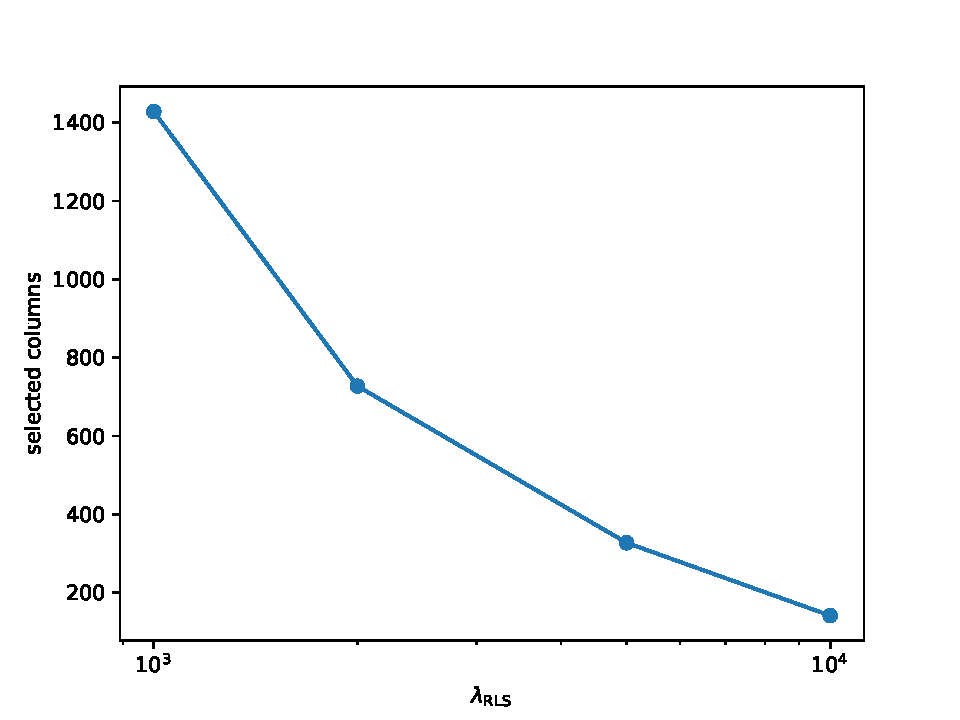
\includegraphics[width=0.72\textwidth]
{Results/final_recursive_lambda_selected_columns.pdf}
\caption{Number of selected recursive RLS columns against $\lambda_{\mathrm{RLS}}$.}
\label{fig:rlc}
\end{figure}
\FloatBarrier

Figure \ref{fig:rlc} shows that increasing $\lambda_{\mathrm{RLS}}$ decreases the number of selected columns. A larger value reduces the effective dimension and therefore lowers the sampling probabilities. In contrast, small values cause the algorithm to return a large number of columns. 

\begin{figure}[h]
\centering
\begin{minipage}{0.49\textwidth}
\centering
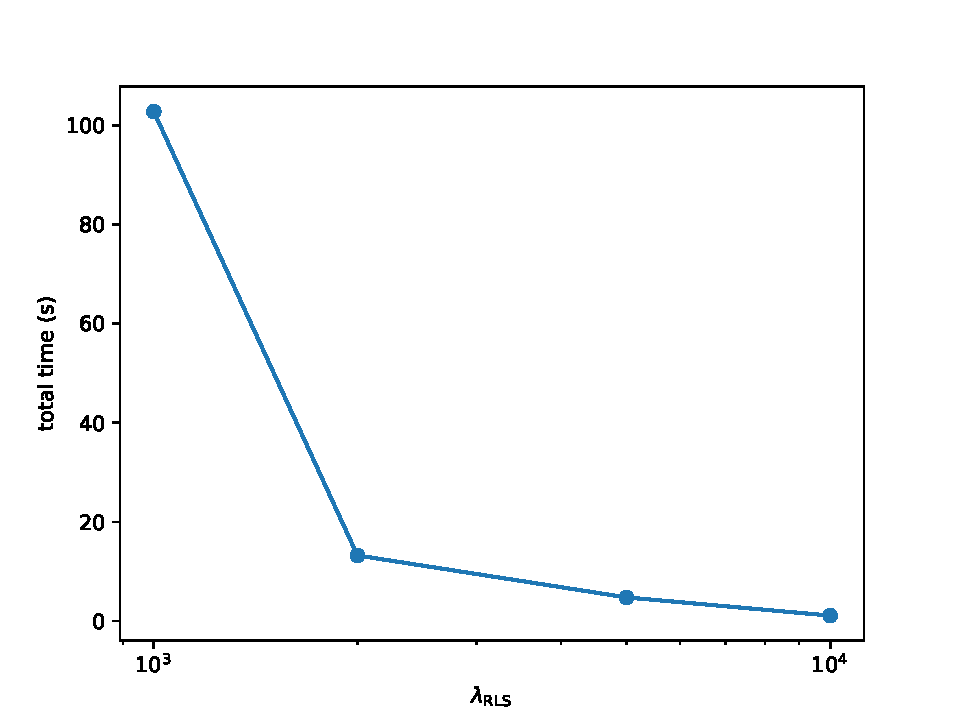
\includegraphics[width=0.98\textwidth]
{Results/final_recursive_lambda_total_time.pdf}
\caption{Recursive RLS total time against
$\lambda_{\mathrm{RLS}}$.}
\label{fig:rlt}
\end{minipage}
\hspace{0.005\textwidth}
\begin{minipage}{0.49\textwidth}
\centering
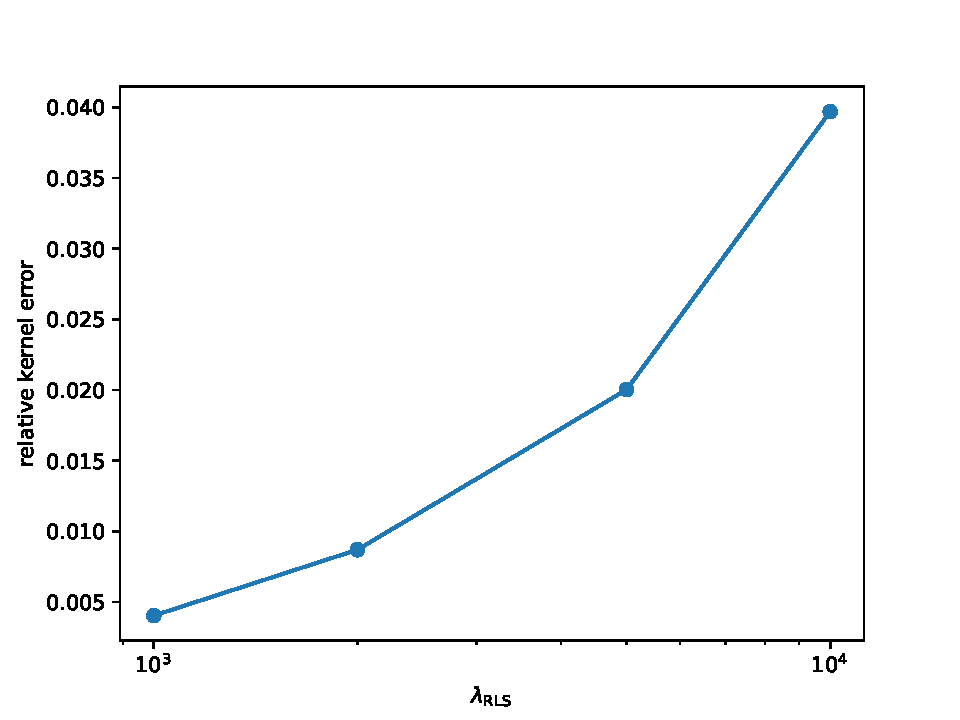
\includegraphics[width=0.98\textwidth]
{Results/final_recursive_lambda_kernel_error.pdf}
\caption{Recursive RLS kernel error against
$\lambda_{\mathrm{RLS}}$.}
\label{fig:rlke}
\end{minipage}
\end{figure}
\FloatBarrier

Figures \ref{fig:rlt} and \ref{fig:rlke} show the resulting trade off. Smaller values of $\lambda_{\mathrm{RLS}}$ select more landmarks and produce a more accurate kernel approximation, but the sampling and factorization costs increase. Larger values select fewer landmarks and reduce runtime, but the kernel approximation error increases.

This completes the discussion on informed column sampling methods. The next section discusses the experimental setup and compares recursive RLS with uniform and approximate leverage sampling using a variety of metrics.